\chapter{Observed dielectron mass distributions}

The observed dielectron invariant mass distributions for the remaining analysis categories not presented in Chapter~\ref{chap:results} are shown in Figure~\ref{fig:app_splusb}.

\begin{figure}[htbp!]
\centering
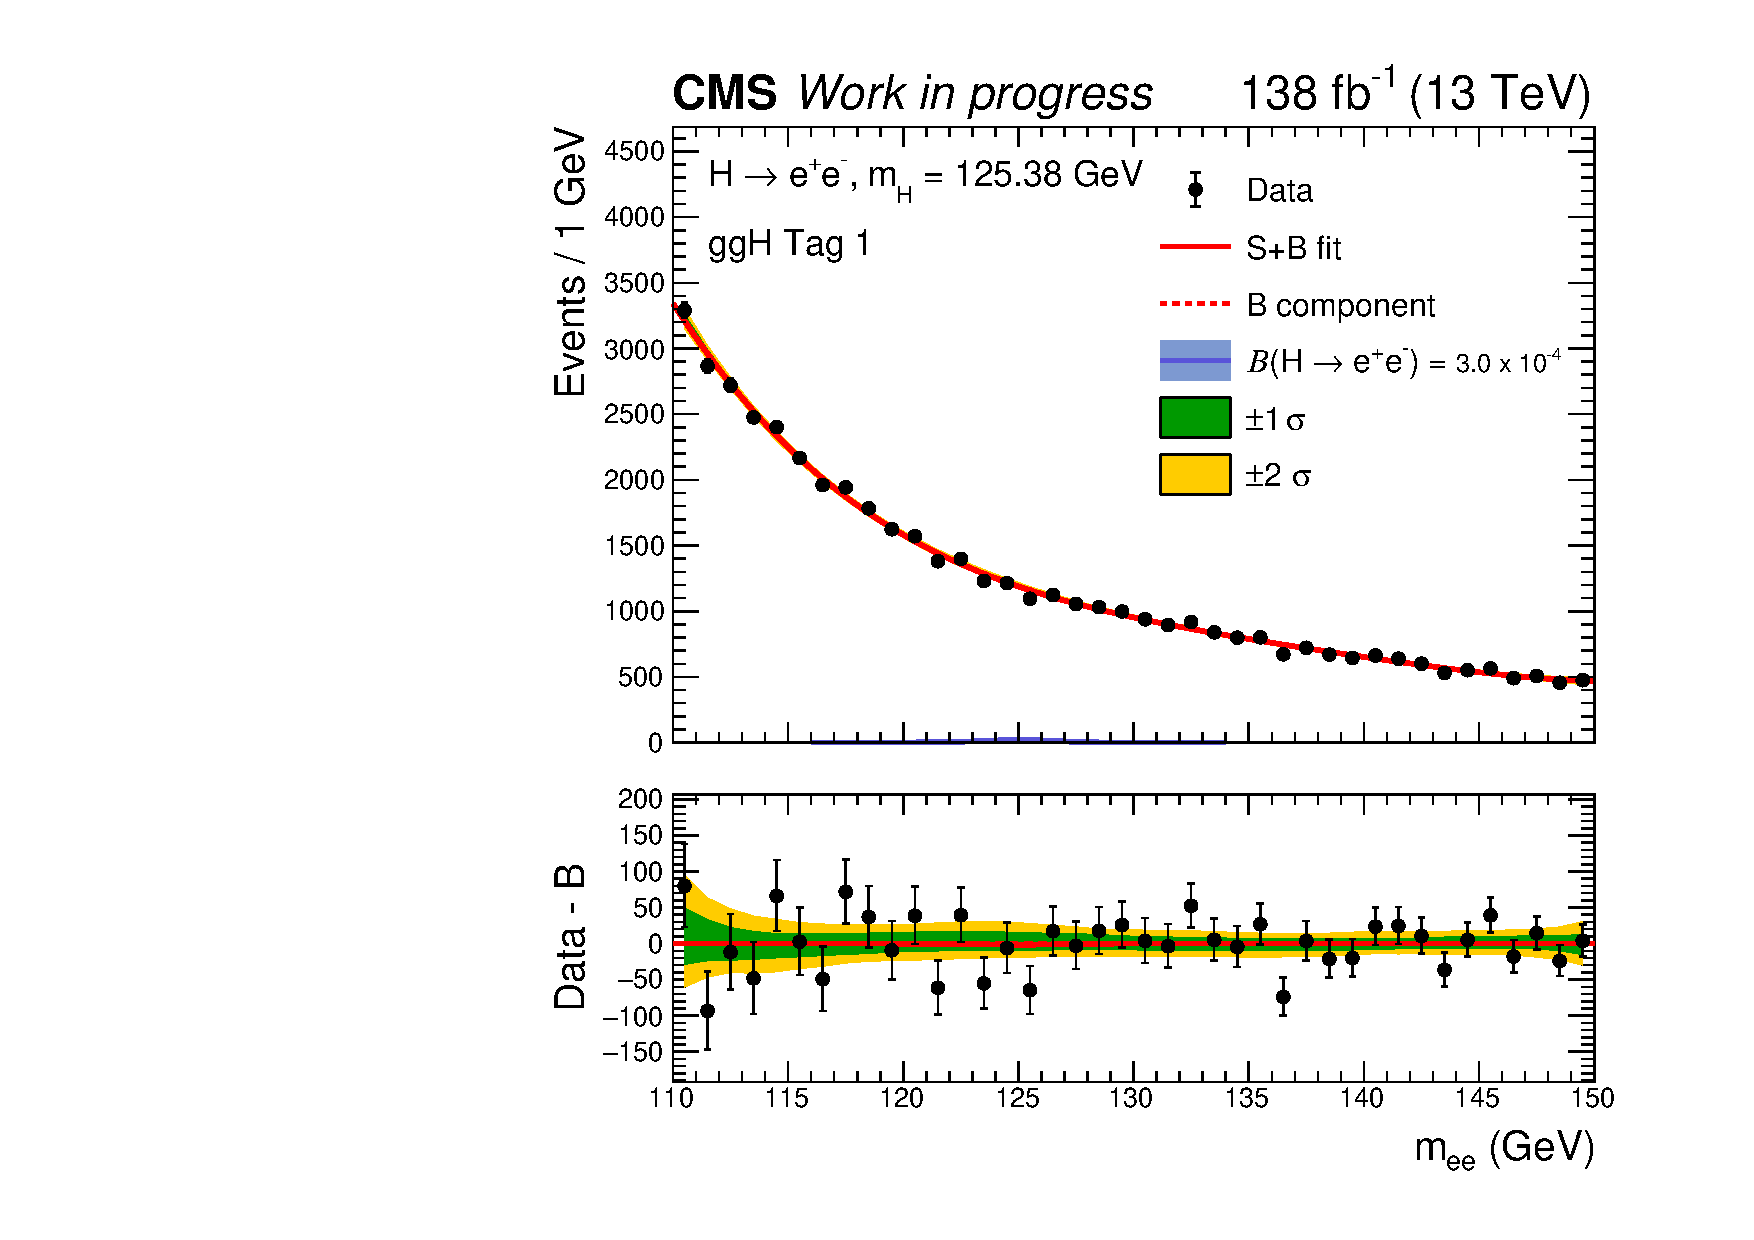
\includegraphics[width =0.46\linewidth]{Figures/Hee/Results/SPlusBModels/gghcat1_CMS_hgg_mass.pdf}\hfill
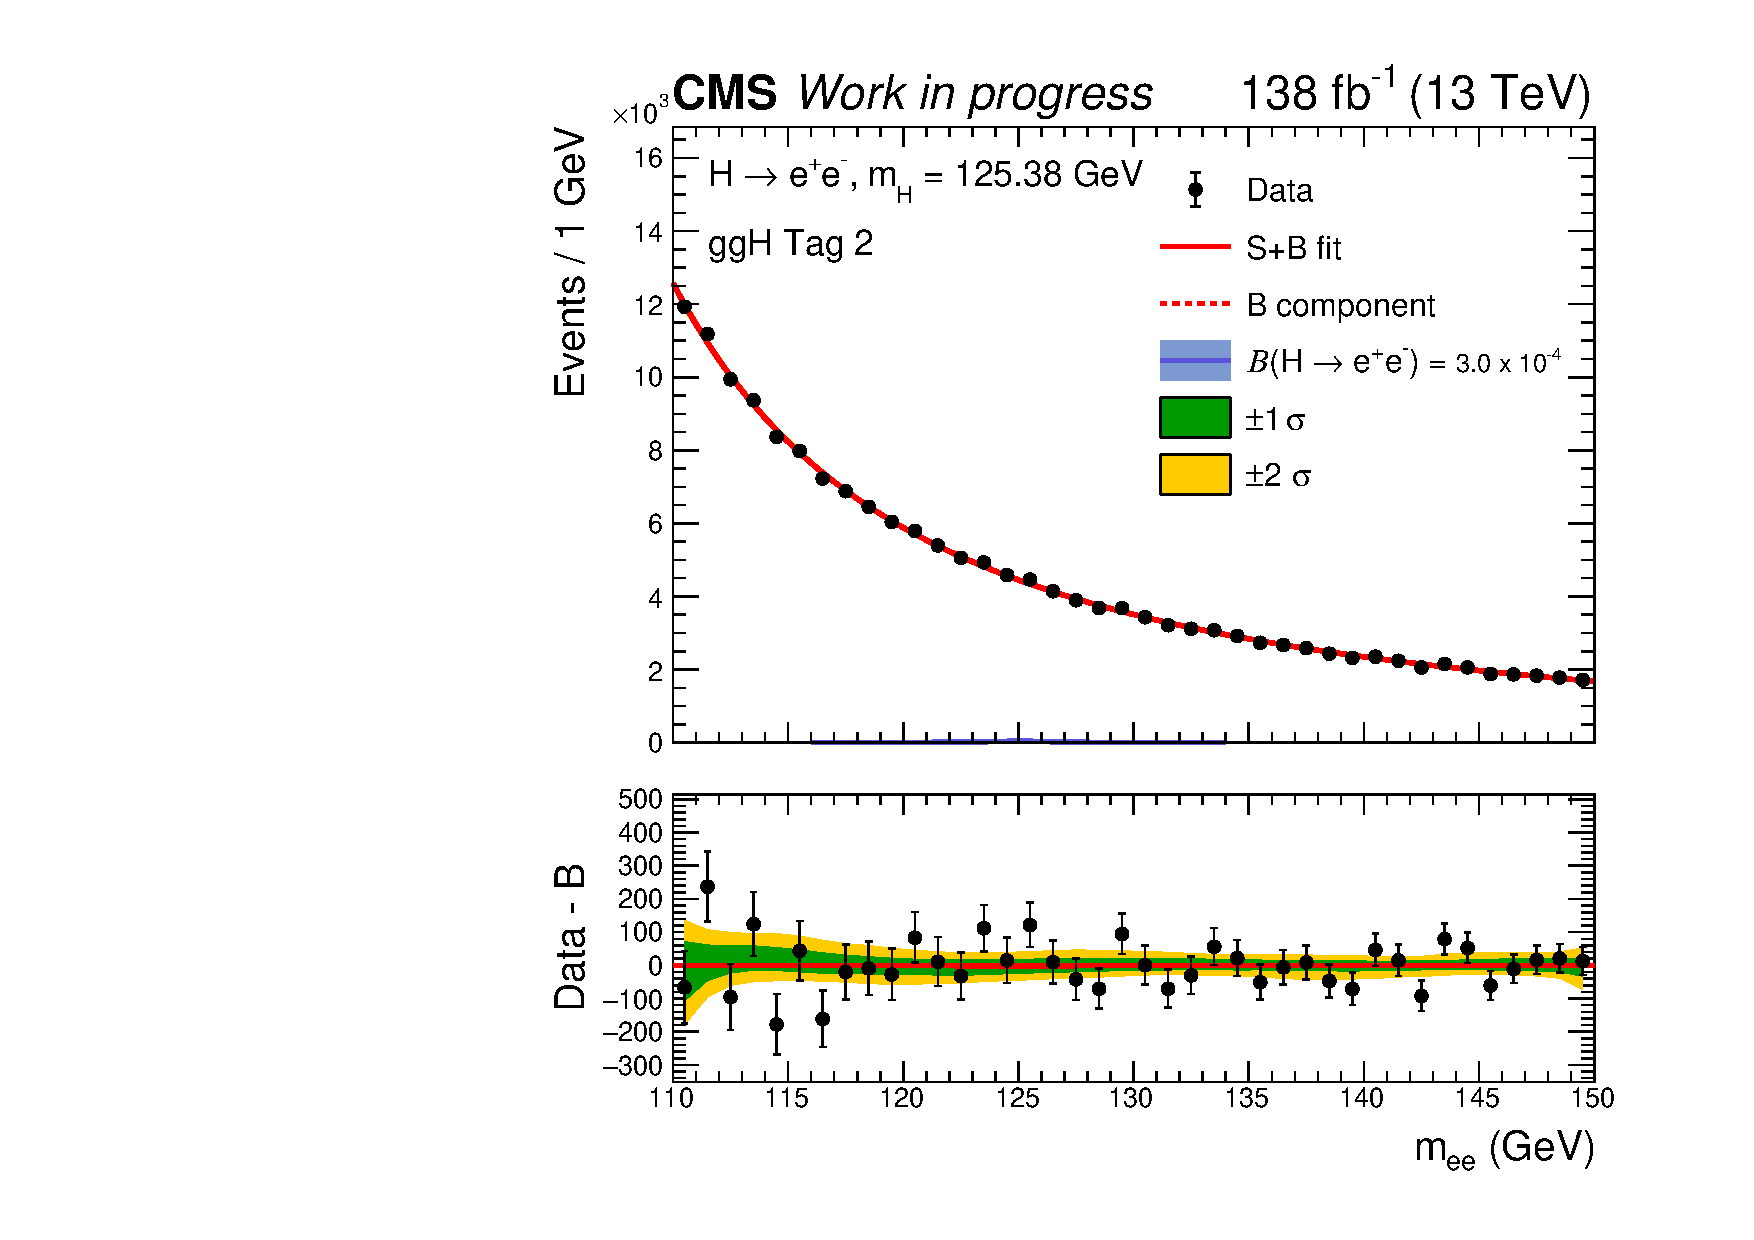
\includegraphics[width =0.46\linewidth]{Figures/Hee/Results/SPlusBModels/gghcat2_CMS_hgg_mass.pdf}\hfill\\%
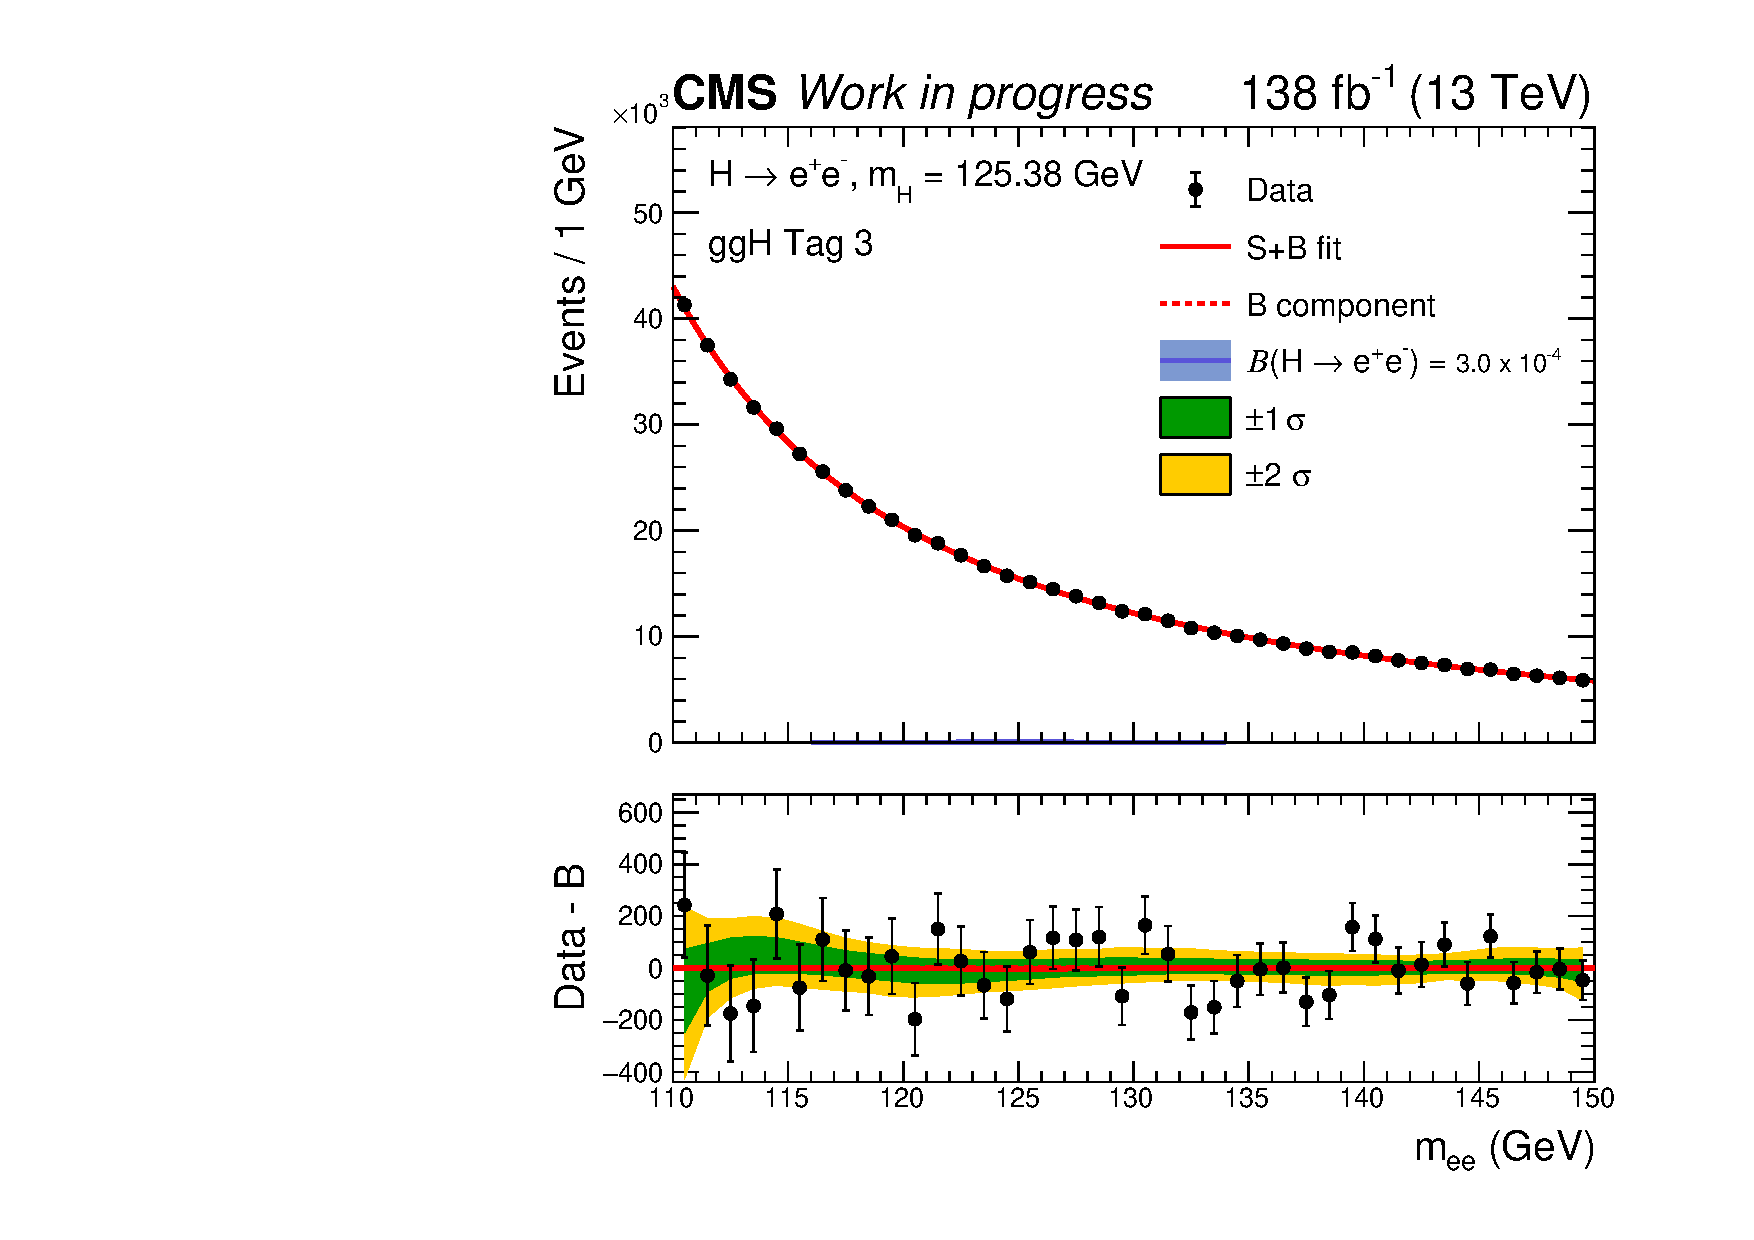
\includegraphics[width =0.46\linewidth]{Figures/Hee/Results/SPlusBModels/gghcat3_CMS_hgg_mass.pdf}\hfill
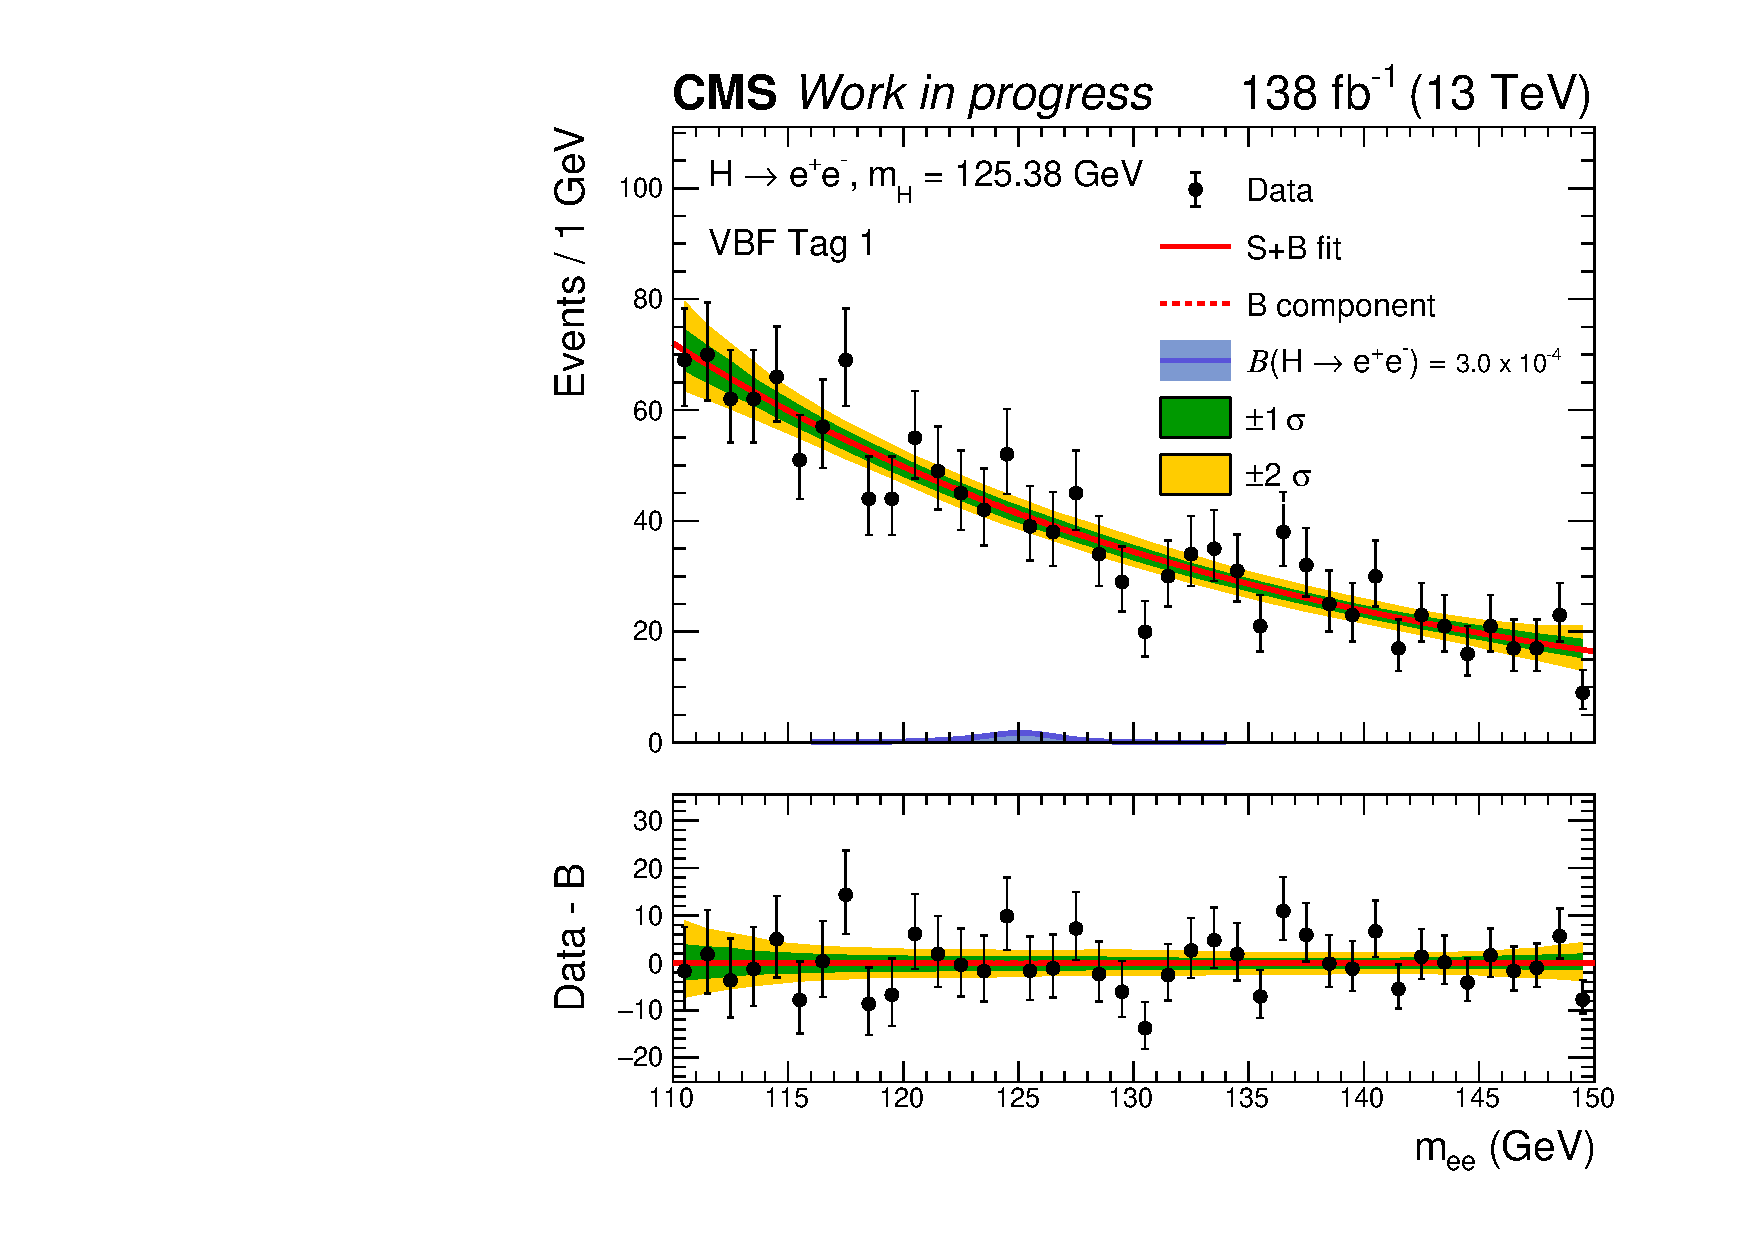
\includegraphics[width =0.46\linewidth]{Figures/Hee/Results/SPlusBModels/vbfcat1_CMS_hgg_mass.pdf}\hfill\\
\caption[The observed dielectron invariant mass distribution for the \ggH Tag 1-3 and VBF Tag 0 analysis categories.]{The dielectron mass distribution for analysis categories targeting \ggH production (Tags 1-3), and categories targeting VBF production (Tag 1). The signal-plus-background model fit to the distributions is shown by the solid red line, while the background only component is shown by the dashed red line. The signal model in each category, shown in blue, is scaled to the expected limit at \mH= 125.38~GeV. The one (green) and two (yellow) standard deviation bands show the uncertainties in the background component of the fit. The lower panel shows the residuals after subtraction of this background component.} 
\label{fig:app_splusb}            
\end{figure}